\documentclass{article}
\usepackage{amsmath,graphicx,mlspconf}

\usepackage{filecontents}
\usepackage[hidelinks,bookmarks=false,draft]{hyperref}
\usepackage{cite}
\usepackage{enumitem}

\usepackage{hyphenat}

\usepackage{setspace}
\usepackage[english]{babel}

\usepackage[hang]{footmisc}

\setlength\footnotemargin{8pt}

\begin{filecontents*}{ESC-CNN.bib}
@article{lecun1989backpropagation,
  title={Backpropagation applied to handwritten zip code recognition},
  author={LeCun, Y. and others},
  journal={Neural computation},
  volume={1},
  number={4},
  pages={541--551},
  year={1989},
  publisher={MIT Press}
}

@article{fukushima1980neocognitron,
  title={Neocognitron: A self-organizing neural network model for a mechanism of pattern recognition unaffected by shift in position},
  author={Fukushima, K.},
  journal={Biological cybernetics},
  volume={36},
  number={4},
  pages={193--202},
  year={1980},
  publisher={Springer}
}

@inproceedings{krizhevsky2012imagenet,
  title={{ImageNet} classification with deep convolutional neural networks},
  author={Krizhevsky, A. and Sutskever, I. and Hinton, G. E.},
  booktitle={Advances in Neural Information Processing Systems},
  pages={1097--1105},
  year={2012}
}

@article{ILSVRC15,
Author = {Russakovsky, O. and others},
Title = {{ImageNet Large Scale Visual Recognition Challenge}},
Year = {2014},
journal = {arXiv preprint arXiv:1409.0575}
}

@article{ciresan2012traffic,
  title={Multi-column deep neural network for traffic sign classification},
  author={Cire{\c{s}}an, D. and Meier, U. and Masci, J. and Schmidhuber, J.},
  journal={Neural Networks},
  volume={32},
  pages={333--338},
  year={2012},
  publisher={Elsevier}
}

@inproceedings{ciresan2012multi,
  title={Multi-column deep neural networks for image classification},
  author={Cire{\c{s}}an, D. and Meier, U. and Schmidhuber, J.},
  booktitle={Proceedings of the IEEE Conference on Computer Vision and Pattern Recognition (CVPR)},
  pages={3642--3649},
  year={2012},
  organization={IEEE}
}

@article{sermanet2013overfeat,
  title={Overfeat: Integrated recognition, localization and detection using convolutional networks},
  author={Sermanet, P. and others},
  journal={arXiv preprint arXiv:1312.6229},
  year={2013}
}

@article{goodfellow2013multi,
  title={Multi-digit number recognition from street view imagery using deep convolutional neural networks},
  author={Goodfellow, I. J. and others},
  journal={arXiv preprint arXiv:1312.6082},
  year={2013}
}

@inproceedings{sermanet2012convolutional,
  title={Convolutional neural networks applied to house numbers digit classification},
  author={Sermanet, P. and Chintala, S. and LeCun, Y.},
  booktitle={Proceedings of the 21st International Conference on Pattern Recognition (ICPR)},
  pages={3288--3291},
  year={2012},
  organization={IEEE}
}

@inproceedings{sermanet2013pedestrian,
  title={Pedestrian detection with unsupervised multi-stage feature learning},
  author={Sermanet, P. and Kavukcuoglu, K. and Chintala, S. and LeCun, Y.},
  booktitle={Proceedings of the IEEE Conference on Computer Vision and Pattern Recognition (CVPR)},
  pages={3626--3633},
  year={2013},
  organization={IEEE}
}

@inproceedings{ciresan2012deep,
  title={Deep neural networks segment neuronal membranes in electron microscopy images},
  author={Cire{\c{s}}an, D. and Giusti, A. and Gambardella, L. M. and Schmidhuber, J.},
  booktitle={Advances in Neural Information Processing Systems},
  pages={2843--2851},
  year={2012}
}

@article{lecun1998gradient,
  title={Gradient-based learning applied to document recognition},
  author={LeCun, Y. and Bottou, L. and Bengio, Y. and Haffner, P.},
  journal={Proceedings of the IEEE},
  volume={86},
  number={11},
  pages={2278--2324},
  year={1998},
  publisher={IEEE}
}

@inproceedings{deng2013recent,
  title={Recent advances in deep learning for speech research at {Microsoft}},
  author={Deng, L. and others},
  booktitle={Proceedings of the IEEE International Conference on Acoustics, Speech and Signal Processing (ICASSP)},
  pages={8604--8608},
  year={2013},
  organization={IEEE}
}

@inproceedings{lee2009unsupervised,
  title={Unsupervised feature learning for audio classification using convolutional deep belief networks},
  author={Lee, H. and Pham, P. and Largman, Y. and Ng, A. Y.},
  booktitle={Advances in Neural Information Processing Systems},
  pages={1096--1104},
  year={2009}
}

@inproceedings{deng2013deep,
  title={A deep convolutional neural network using heterogeneous pooling for trading acoustic invariance with phonetic confusion},
  author={Deng, L. and Abdel-Hamid, O. and Yu, D.},
  booktitle={Proceedings of the IEEE International Conference on Acoustics, Speech and Signal Processing (ICASSP)},
  pages={6669--6673},
  year={2013},
  organization={IEEE}
}

@article{abdel2014convolutional,
  title={Convolutional neural networks for speech recognition},
  author={Abdel-Hamid, O. and others},
  journal={IEEE/ACM Transactions on Audio, Speech and Language Processing (TASLP)},
  volume={22},
  number={10},
  pages={1533--1545},
  year={2014},
  publisher={IEEE Press}
}

@inproceedings{sainath2013deep,
  title={Deep convolutional neural networks for {LVCSR}},
  author={Sainath, T. N. and Mohamed, A. and Kingsbury, B. and Ramabhadran, B.},
  booktitle={Proceedings of the IEEE International Conference on Acoustics, Speech and Signal Processing (ICASSP)},
  pages={8614--8618},
  year={2013},
  organization={IEEE}
}

@inproceedings{abdel2012applying,
  title={Applying convolutional neural networks concepts to hybrid {NN-HMM} model for speech recognition},
  author={Abdel-Hamid, O. and Mohamed, A. and Jiang, H. and Penn, G.},
  booktitle={Proceedings of the IEEE International Conference on Acoustics, Speech and Signal Processing (ICASSP)},
  pages={4277--4280},
  year={2012},
  organization={IEEE}
}

@inproceedings{abdel2013exploring,
  title={Exploring convolutional neural network structures and optimization techniques for speech recognition},
  author={Abdel-Hamid, O. and Deng, L. and Yu, D.},
  booktitle={Proceedings of INTERSPEECH},
  pages={3366--3370},
  year={2013}
}

@inproceedings{van2013deep,
  title={Deep content-based music recommendation},
  author={Van den Oord, A. and Dieleman, S. and Schrauwen, B.},
  booktitle={Advances in Neural Information Processing Systems},
  pages={2643--2651},
  year={2013}
}

@inproceedings{dieleman2011audio,
  title={Audio-based Music Classification with a Pretrained Convolutional Network},
  author={Dieleman, S. and Brakel, P. and Schrauwen, B.},
  booktitle={Proceedings of the 12th International Society for Music Information Retrieval (ISMIR) conference},
  pages={669--674},
  year={2011}
}

@article{chachada2014environmental,
  title={Environmental sound recognition: A survey},
  author={Chachada, S. and Kuo, C.-C. J.},
  journal={APSIPA Transactions on Signal and Information Processing},
  volume={3},
  pages={e14},
  year={2014},
  publisher={Cambridge Univ Press}
}

@article{barchiesi2015acoustic,
  title={Acoustic Scene Classification: Classifying environments from the sounds they produce},
  author={Barchiesi, D. and Giannoulis, D. and Stowell, D. and Plumbley, M. D.},
  journal={Signal Processing Magazine},
  volume={32},
  number={3},
  pages={16--34},
  year={2015},
  publisher={IEEE}
}


@inproceedings{asgari2014inferring,
  title={Inferring social contexts from audio recordings using deep neural networks},
  author={Asgari, M. and Shafran, I. and Bayestehtashk, A.},
  booktitle={Proceedings of the IEEE International Workshop on Machine Learning for Signal Processing (MLSP)},
  year={2014},
  organization={IEEE}
}

@inproceedings{kons2013audio,
  title={Audio event classification using deep neural networks},
  author={Kons, Z. and Toledo-Ronen, O.},
  booktitle={Proceedings of INTERSPEECH},
  pages={1482--1486},
  year={2013}
}

@inproceedings{ravanelli2014audio,
  title={Audio Concept Classification with Hierarchical Deep Neural Networks},
  author={Ravanelli, M. and Elizalde, B. and Ni, K. and Friedland, G.},
  booktitle={Proceedings of the 22nd European Signal Processing Conference (EUSIPCO)},
  pages={606--610},
  year={2014},
  organization={IEEE}
}

@inproceedings{gencoglu2014recognition,
  title={Recognition of acoustic events using deep neural networks},
  author={Gencoglu, O. and Virtanen, T. and Huttunen, H.},
  booktitle={Proceedings of the 22nd European Signal Processing Conference (EUSIPCO)},
  pages={506--510},
  year={2014},
  organization={IEEE}
}

@inproceedings{xue2015auditory,
  title={Auditory Scene Classification with Deep Belief Network},
  author={Xue, L. and Su, F.},
  booktitle={MultiMedia Modeling},
  pages={348--359},
  year={2015},
  organization={Springer}
}

@article{hinton2012improving,
  title={Improving neural networks by preventing co-adaptation of feature detectors},
  author={Hinton, G. E. and others},
  journal={arXiv preprint arXiv:1207.0580},
  year={2012}
}

@inproceedings{salamon2014dataset,
  title={A Dataset and Taxonomy for Urban Sound Research},
  author={Salamon, J. and Jacoby, C. and Bello, J. P.},
  booktitle={Proceedings of the ACM International Conference on Multimedia},
  pages={1041--1044},
  year={2014},
  organization={ACM}
}

@inproceedings{piczak2015esc,
  title={{ESC}: Dataset for Environmental Sound Classification},
  author={Piczak, K. J.},
  booktitle={Proceedings of the ACM International Conference on Multimedia},
  year={2015},
  organization={ACM},
  note={in press}
}

@inproceedings{salamon2015unsupervised,
  title={Unsupervised feature learning for urban sound classification},
  author={Salamon, J. and Bello, J. P.},
  booktitle={Proceedings of the IEEE International Conference on Acoustics, Speech and Signal Processing (ICASSP)},
  year={2015}
}

@inproceedings{glorot2011deep,
  title={Deep sparse rectifier neural networks},
  author={Glorot, X. and Bordes, A. and Bengio, Y.},
  booktitle={Proceedings of the 14th International Conference on Artificial Intelligence and Statistics. JMLR W\&CP},
  volume={15},
  pages={315--323},
  year={2011}
}

@article{xu2015empirical,
  title={Empirical Evaluation of Rectified Activations in Convolutional Network},
  author={Xu, B. and Wang, N. and Chen, T. and Li, M.},
  journal={arXiv preprint arXiv:1505.00853},
  year={2015}
}

@inproceedings{maas2013rectifier,
  title={Rectifier nonlinearities improve neural network acoustic models},
  author={Maas, A. L. and Hannun, A. Y. and Ng, A. Y.},
  booktitle={ICML Workshop on Deep Learning for Audio, Speech, and Language Processing},
  year={2013}
}

@inproceedings{bengio2013advances,
  title={Advances in optimizing recurrent networks},
  author={Bengio, Y. and Boulanger-Lewandowski, N. and Pascanu, R.},
  booktitle={Proceedings of the IEEE International Conference on Acoustics, Speech and Signal Processing (ICASSP)},
  pages={8624--8628},
  year={2013},
  organization={IEEE}
}

@book{yu2015deeplearning,
author = {Yu, D. and Deng, L.},
title = {Automatic Speech Recognition: A Deep Learning Approach},
publisher = {Springer},
year = {2014},
}

@book{bengio2015deeplearning,
    title={Deep Learning},
    author={Bengio, Y. and Goodfellow, I. J., and Courville, A.},
    note={Book in preparation for MIT Press},
    url={http://www.iro.umontreal.ca/~bengioy/dlbook},
    year={2015}
}

@book{deng2014deep,
  title={Deep Learning: Methods and Applications},
  author={Deng, L. and Yu, D.},
  year={2014},
  publisher={{NOW Publishers}}
}

@article{pylearn2,
    author = {Goodfellow, I. J. and others},
     title = {Pylearn2: a machine learning research library},
   journal = {arXiv preprint arXiv:1308.4214},
      year = {2013},	
       url = {http://arxiv.org/abs/1308.4214},
}

\end{filecontents*}

\copyrightnotice{978-1-4673-7454-5/15/\$31.00 {\copyright}2015 IEEE}

\toappear{2015 IEEE International Workshop on Machine Learning for Signal Processing, Sept.\ 17--20, 2015, Boston, USA}

\title{Environmental Sound Classification\\with Convolutional Neural Networks}

\name{Karol J. Piczak}
\address{Institute of Electronic Systems\\
		 Warsaw University of Technology}

\begin{document}
\maketitle

\lefthyphenmin=2
\righthyphenmin=3
\tolerance=400
\emergencystretch=12pt
\hyphenpenalty=700

\begin{abstract}
This paper evaluates the potential of convolutional neural networks in classifying short audio clips of environmental sounds. A deep model consisting of 2 convolutional layers with max-pooling and 2 fully connected layers is trained on a low level representation of audio data (segmented spectrograms) with deltas. The accuracy of the network is evaluated on 3 public datasets of environmental and urban recordings. The model outperforms baseline implementations relying on mel-frequency cepstral coefficients and achieves results comparable to other state-of-the-art approaches.
\end{abstract}

\begin{keywords}
environmental sound, convolutional neural networks, classification
\end{keywords}

\section{Introduction}

Convolutional neural networks date back as far as to the 1980s~\cite{fukushima1980neocognitron,  lecun1989backpropagation, lecun1998gradient}, yet only recently have they been adopted as a~method of choice for various object classification tasks. The work of Krizhevsky et~al.~\cite{krizhevsky2012imagenet} marked a~turning point in large scale visual recognition \cite{ILSVRC15} in 2012. Since then, by replacing techniques relying on manually engineered features, convolutional neural networks allowed for significant progress in numerous pattern recognition tasks, including classification of traffic signs~\cite{ciresan2012traffic}, house numbers~\cite{goodfellow2013multi, sermanet2012convolutional} and handwritten digits~\cite{ciresan2012multi}, pedestrian detection~\cite{sermanet2013pedestrian}, and electron microscopy image processing~\cite{ciresan2012deep}.

Although primarily used in visual recognition contexts, convolutional architectures have been also successfully applied in speech~\cite{lee2009unsupervised, deng2013deep, abdel2014convolutional, sainath2013deep, abdel2012applying, abdel2013exploring, deng2013recent} and music analysis~\cite{dieleman2011audio, van2013deep}. These efforts have shown that approaches taking advantage of data locality can provide viable solutions to problems encountered in other domains. A thorough coverage of current deep learning methods and their applications in various contexts, including speech and audio processing, can be found in recently published books discussing this topic~\cite{bengio2015deeplearning, yu2015deeplearning, deng2014deep}.

At the same time, classification of environmental sounds (everyday audio events that do not consist of music or speech data and are often more diverse and chaotic in their structure) is still predominantly based on applying general classifiers (Gaussian mixture models, support vector machines, hidden Markov models) to manually extracted features, such as mel-frequency cepstral coefficients. Recent reviews pertaining to this subject~\cite{barchiesi2015acoustic, chachada2014environmental} present a detailed analysis of the most common approaches. The introduction of deep learning techniques in this context has slowly begun in the last two years. However, these efforts are still mostly limited to analyzing highly pre-processed acoustic features~\cite{asgari2014inferring, kons2013audio, ravanelli2014audio, gencoglu2014recognition, xue2015auditory}.

This contrast in the development of different fields raises a research question which has not yet been widely addressed. \textit{Can convolutional neural networks be effectively used in classifying environmental and urban sound sources}? The goal of this paper is to provide an answer to this question.

\vspace{-6pt}

\section{Convolutional neural networks}

In essence, convolutional neural networks are a simple extension of the multilayer perceptron model. However, their architectural differences have significant practical consequences.

\vspace{-6pt}

\subsection{Layer architecture}

\begin{figure}
\centering
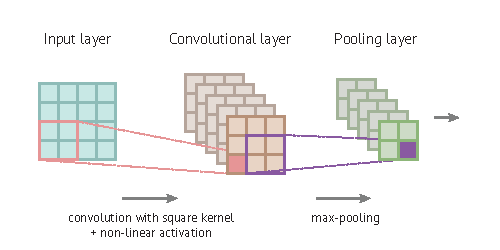
\includegraphics[width=20pc]{Figures/ConvLayer.pdf}
\caption{\label{fig:convolutional-layer}A schematic visualization of a typical convolution-pooling operation performed on the input data.}
\end{figure}

A typical convolutional neural network consists of a number of different layers stacked together in a deep architecture: an input layer, a group of convolutional and pooling layers (which can be combined in various ways), a limited number of fully connected hidden layers, and an output (loss) layer. The actual difference, when compared to the multilayer perceptron, lies in the introduction of a combination of convolution and pooling operations (depicted in Figure~\ref{fig:convolutional-layer}).

A convolutional layer introduces a special way of organizing hidden units which aims to take advantage of the local structure present in the two-dimensional input data (mostly, but not limited to, images). Each hidden unit, instead of being connected to all the inputs coming from the previous layer, is limited to processing only a tiny part of the whole input space (e.g. small $3\times3$ blocks of pixels), called its \textit{receptive field}. The weights of such a hidden unit create a~\textit{convolutional kernel} (\textit{filter}) which is applied to (tiled over) the whole input space, resulting in a \textit{feature map}. This way, one set of weights can be reused for the whole input space. This is based on the premise that locally useful features will be also useful in other places of the input space - a mechanism which not only vastly reduces the number of parameters to estimate, but improves robustness to translational shifts of the data. A typical convolutional layer will consist of numerous \textit{filters} (\textit{feature maps}).

Further dimensionality reduction can be achieved through \textit{pooling} layers, which merge adjacent cells of a feature map. The most common pooling operations performed are taking the \textit{max} (winner takes all) or \textit{mean} of the input cells. This downsampling further improves invariance to translations.

\subsection{Rectified Linear Units}

Traditionally, logistic sigmoid and hyperbolic tangent have been used as typical non-linear activation functions in a multilayer perceptron setup. Recent implementations of deep architectures have unequivocally replaced them with alternative solutions. One of the most common is the application of \textit{Rectified Linear Units} (ReLUs), which use the following activation function:

\vspace{-6pt}

\begin{equation}
f(x) = max(0, x)
\end{equation}

ReLUs have several advantages over traditional units: faster computation and more efficient gradient propagation (they do not saturate as is the case with sigmoid units), biological plausibility (one-sidedness) and sparse activation structure \cite{glorot2011deep}, while still retaining sufficient discriminatory properties despite their simplicity. One of their drawbacks is that depending on the state of the random weight initialization, multiple units may prematurely fall into the ``dead zone'' - outputting a constant gradient of zero. For this reason, alternatives with a non-zero slope such as \textit{Leaky Rectified Linear Units} have been suggested~\cite{maas2013rectifier}, and empirical results seem to confirm their usefulness~\cite{xu2015empirical}.

\subsection{Dropout learning}

Deep neural architectures have a natural tendency to overfitting. Even in convolutional neural networks, where the quantity of parameters is reduced through weight sharing, the number of estimated values is most of the times bigger than the number of training cases by an order of magnitude. This can result in poor out-of-sample generalization.

One way to tackle this problem was introduced in the form of \textit{dropout} learning~\cite{hinton2012improving}. The concept is quite simple, yet highly effective. In each training iteration every hidden unit is randomly removed with a predefined probability (originally 50\%), and the learning procedure continues normally. These random perturbations effectively prevent the network from learning spurious dependencies, and creating complex co-adaptations between hidden units. This way big groups of neurons become helpful not only in the context of other neurons. Architecture averaging introduced by dropout tries to ensure that each hidden unit learns feature representations that are generally favorable in producing the correct classification answer. 

\vspace{-12pt}

\section{Sound classification}

\subsection{Datasets}

One of the main problems with training deep neural architectures in a supervised manner is the amount of computational effort and labeled data required for efficient learning. While the former is in some part addressed on a universal basis by hardware advances and general-purpose GPU computing, the latter is very domain-dependent.

Unfortunately, publicly available datasets of environmental recordings are still very limited - both in number and in size\footnote{A list of datasets in this field is currently maintained by Toni Heittola at:\\\urlstyle{same}\url{http://www.cs.tut.fi/~heittolt/datasets} [\textit{last accessed: July 30, 2015}].}. This is quite understandable, considering the high cost of manual annotation. Although the situation gradually improves with the introduction of new collections of recordings~\cite{salamon2014dataset, piczak2015esc}, it is still one of the major hindrances to the development of new data-intensive approaches in this field. This is especially important, since the performance of supervised deep models is strongly influenced by the size of the dataset available for learning. Therefore, the original research problem has to be extended in this context - \textit{can convolutional neural networks be effectively used for environmental sound classification with limited amount of training data}?

To answer this question, three publicly available datasets were selected for evaluation of the models: \textit{ESC-50}~\cite{piczak2015esc}, \textit{ESC-10}~\cite{piczak2015esc} and \textit{UrbanSound8K}~\cite{salamon2014dataset}.

The \textit{ESC-50} dataset is a collection of 2000 short (5 seconds) environmental recordings comprising 50 equally balanced classes of sound events in 5 major groups (animals, natural soundscapes and water sounds, human non-speech sounds, interior/domestic sounds, and exterior/urban noises) prearranged into 5 folds for comparable cross-validation. It~is a demanding compilation with baseline approaches (classification with random forest ensemble using features derived from mel-frequency cepstral coefficients and zero-crossing rate) achieving a mean accuracy of 44\%, and recognition accuracy of untrained human participants at approximately 81\%~\cite{piczak2015esc}.

\textit{ESC-10} is a less complex standardized subset of 10~classes (400 recordings) selected from the \textit{ESC-50} dataset (\textit{dog bark}, \textit{rain}, \textit{sea waves}, \textit{baby cry}, \textit{clock tick}, \textit{person sneeze}, \textit{helicopter}, \textit{chainsaw}, \textit{rooster}, \textit{fire crackling}). Using the same implementations of the baseline classifier yields an accuracy of 73\% (5 fold cross-validation), with respective human benchmark of 96\%~\cite{piczak2015esc}.

\textit{UrbanSound8K} is a collection of 8732 short (less than 4~seconds) excerpts of various urban sound sources (\textit{air conditioner}, \textit{car horn}, \textit{playing children}, \textit{dog bark}, \textit{drilling}, \textit{engine idling}, \textit{gun shot}, \textit{jackhammer}, \textit{siren}, \textit{street music}) prearranged into 10 folds. Based on this dataset, the work of Salamon and Bello~\cite{salamon2015unsupervised} compares a baseline system with unsupervised feature learning performed on patches of PCA-whitened log-scaled mel-spectrograms. The average classification accuracy obtained is respectively 68\% for the baseline and 73.6\% for the best performing variant of the evaluated system.

\subsection[Experiment setup]{Experiment setup\footnote{Source code for study replication is available as an IPython notebook at:\\\href{https://github.com/karoldvl/paper-2015-esc-convnet}{https://github.com/karoldvl/paper-2015-esc-convnet}.}}

\begin{figure}[!t]
\centering
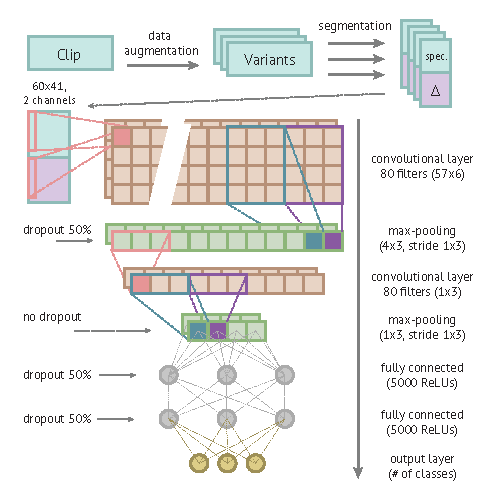
\includegraphics[width=20pc]{Figures/Architecture.pdf}
\caption{\label{fig:architecture}Model architecture for the short segment variation.}
\end{figure}

Training a convolutional neural network involves a lot of decisions that have to be made regarding both the architecture (format of the input data, number and size of layers, amount of spatial pooling, filter dimensions) and learning hyperparameters (learning rate, momentum, batch size, dropout probability, amount of regularization applied). This selection process is still mostly based on heuristics, especially when entering uncharted territories of new applications.

Due to the time required for training a complete model, exhaustive evaluation of all potential combinations was infeasible. Therefore, the selection of the most promising model had to be based on limited validation (single fold) performed for most significant factors (number of layers/filters, filter shape, learning rate, dropout probability). The final system that was evaluated in detail can be described through the following process depicted in Figure~\ref{fig:architecture}:

\begin{itemize}[noitemsep,topsep=0pt,leftmargin=12pt]
\itemsep0em
\item The \textit{ESC-50} and \textit{ESC-10} training datasets were augmented by applying random time delays to the original recordings. Additionally, class-dependent time-stretching and pitch-shifting was performed on the \textit{ESC-10} training set. 10 augmentations were created for each clip of the \textit{ESC-10} dataset and 4 variants for the \textit{ESC-50}. Simple augmentation techniques proved to be unsatisfactory for the \textit{UrbanSound8K} dataset given the considerable increase in training time they generated and negligible impact on model accuracy.

\item Log-scaled mel-spectrograms were extracted from all recordings (resampled to 22050~Hz and normalized) with window size of 1024, hop length of 512 and 60 mel-bands, using the \textit{librosa} implementation\footnote{\textit{librosa: v0.3.1} library by B. McFee et al., DOI: \href{http://dx.doi.org/10.5281/zenodo.12714}{10.5281/zenodo.12714}}.

\item As learning on whole clips was too limiting on the number of examples available for training, the spectrograms were split into 50\% overlapping segments of 41 frames (short variant, segments of approx. 950~ms) or 101 frames with 90\% overlap (long variant, approx.~2.3~s), discarding silent segments in the process.

\item Segments (e.g. 60 rows/bands $\times$ 41 columns/frames) were provided together with their deltas (computed with default \textit{librosa} settings) as a 2-channel input to the network.

\item The first convolutional ReLU layer consisted of 80 filters of rectangular shape (57$\times$6 size, 1$\times$1 stride) allowing for slight frequency invariance. Max-pooling was applied with a pool shape of 4$\times$3 and stride of 1$\times$3. A small selection of learned filters is presented in Figure~\ref{fig:filters}.

\begin{figure}[!h]
\vspace{-6pt}
\centering
\includegraphics[width=20pc]{Figures/Filters.pdf}
\caption{\label{fig:filters}A selection of filters learned by the first convolutional layer.}
\end{figure}

\begin{figure*}
\centering
\includegraphics[width=42pc]{Figures/Results.pdf}
\caption{\label{fig:results}Comparison of classification accuracy on the evaluated datasets.}
\end{figure*}

\item A second convolutional ReLU layer consisted of 80 filters (1$\times$3 size, 1$\times$1 stride) with max-pooling (1$\times$3 pool size, 1$\times$3 pool stride).

\item Further processing was applied through two fully connected hidden layers of 5000 ReLUs each and a softmax output layer.

\item Training was performed using \textit{pylearn2}~\cite{pylearn2} implementation of mini-batch (stochastic) gradient descent with even shuffled sequential batches (batch size of 1000), Nesterov momentum of 0.9~\cite{bengio2013advances}, 0.001 L2 weight decay for each layer and 0.5 dropout probability for fully connected layers and the first convolutional layer.

\item Training procedure was stopped after 300 epochs for the short segment variant (learning rate of 0.002) and 150 epochs for the long variant (learning rate 0.01).

\item Final predictions for a clip were generated using either a~majority-voting scheme or by taking into account the probabilities predicted for each segment.

\end{itemize}

\vspace{-12pt}

\subsection{Results}

\begin{figure}[!hb]
\vspace{-18pt}
\centering
\includegraphics[width=20pc]{Figures/Conf.pdf}
\vspace{-6pt}
\caption{\label{fig:confmatrix}Confusion matrix for the (LP) model evaluated on the \textit{UrbanSound8K} dataset. Classes: air conditioner (AI), car horn (CA), children playing (CH), dog bark (DO), drilling (DR), engine idling (EN), gun shot (GU), jackhammer (JA), siren (SI), street music (ST). See~\cite{salamon2015unsupervised} for comparison.}
\end{figure}

The model was evaluated in a 5-fold (\textit{ESC-10} and \textit{ESC-50}) and 10-fold (\textit{UrbanSound8K}) cross-validation regime with a~single training fold used as an intermittent validation set. Figure~\ref{fig:results} presents classification accuracy achieved by variants of the evaluated model and baseline implementations, with mean accuracy across folds indicated by diamond marks.

\tolerance=500
\hyphenpenalty=250

In all cases models based on a convolutional neural network performed better than respective implementations using manually-engineered features, especially when classifying audio events from more varied categories of the \textit{ESC-50} dataset (baseline accuracy: 44\%, best network: 64.5\%). Models working on longer time scales also seemed to offer slight improvements over variants operating on shorter segments. Unfortunately, further extensions of segment length would most probably be counter-balanced by diminishing returns due to overfitting, as they drastically reduce the effective number of training examples. The probability-voting scheme proved to be universally favorable as compared to a~majority-voting setup.

However, owing to the fact that the presented baselines should be treated as most common approaches and not fine-tuned state-of-the-art techniques, the real potential of convolutional neural networks would still require further evaluation. Nonetheless, a convolutional model using long segments and probability voting achieves results comparable to other best performing models on the \textit{UrbanSound8K} dataset (LP - 73.1\%, US - 73.7\%) with smaller dispersion. 

The model's confusion matrix for the \textit{UrbanSound8K} dataset (Fig.~\ref{fig:confmatrix}), when compared with its analogue for the unsupervised technique presented by Salamon~\&~Bello~\cite{salamon2015unsupervised}, shows some complementary characteristics. The convolutional network performs considerably better in recognizing specific classes (\textit{air conditioner}, \textit{car horn}, \textit{playing children}, \textit{dog bark}) while at the same time performing relatively poor for sounds with short-scale temporal structure (\textit{drilling}, \textit{engine idling}, \textit{jackhammer}). This could indicate that ensemble averaging of different approaches (both convolutional and non-convolutional) may yield even more efficient systems.

\section{Summary}

The goal of this paper was to evaluate whether convolutional neural networks can be successfully applied to environmental sound classification tasks, especially considering the limited nature of datasets available in this field.

\lefthyphenmin=3

It seems that they are indeed a viable solution to this problem. Conducted experiments show that a convolutional model outperforms common approaches based on manually-engineered features and achieves a similar level as other feature learning methods. Although, taking into consideration much longer training times, the result is far from groundbreaking, it shows that convolutional neural networks can be effectively applied in environmental sound classification tasks even with limited datasets and simple data augmentation. What is more, it is quite likely that a considerable increase in the size of the available dataset would vastly improve the performance of trained models, as the gap to human accuracy is still profound.

One of the possible questions open for future inquiry is whether convolutional neural networks could be effectively used in ensembles with other less complex models, as they seem to concentrate on distinct aspects of sound events.

\vspace{-8pt}

\subsubsection*{Acknowledgments}

I would like to thank Justin Salamon for providing details on the results obtained on the \textit{UrbanSound8K} dataset~\cite{salamon2015unsupervised}.


\begin{spacing}{0.94}

\bibliographystyle{IEEEbib}
\bibliography{ESC-CNN}

\end{spacing}

\end{document}